On cherche à modéliser le comportement magnétique d’un cristal ionique constitué de $N$ ions
de spin 1 en équilibre avec un thermostat à la température $T$. Le cristal est plongé dans un champ
magnétique uniforme $\Vec{B}$ dirigé selon un axe ($Oz$). On rappelle que dans ce cas l'énergie d'un ion
de moment magnétique $\Vec{\mu}$  dans le champs $\Vec{B}$ s’écrit $-\Vec{\mu} \cdot \Vec{B}= - \mu_z B$ où $\mu_z$, la projection de
$\Vec{\mu}$ sur l’axe ($Oz$) prend l’une des trois valeurs possibles $ - \mu, 0$ ou $\mu$ ($\mu >0$). Le moment magnétique total $\Vec{M}$ du cristal est la somme des moments magnétiques individuels. Dans la suite, on s’intéresse uniquement aux propriétés magnétiques
du cristal et on ne prend pas en compte l'énergie cinétique des ions ni les vibrations du réseau cristallin.

\tiret{Ions magnétiques sans interactions}

Dans un premier temps, on traite le cristal comme une assemblée de $N$ ions magnétiques sans interactions.
\question  Comment s'écrit alors la fonction de partition canonique $Z(T, N)$  des degrés de liberté magnétiques du système en fonction de $z(T)$, fonction de partition d’un seul ion ?
Pourquoi les ions peuvent-ils être considérés comme discernables ?

\question Calculer $z(T)$.

\question En déduire les probabilités de chacune des orientations du spin 1, puis la moyenne du spin d'un ion.

\question Montrer que le moment magnétique moyen selon $(Oz)$ s'exprime comme $M_z=N\mu \frac{2 \sinh{(\beta \epsilon)}}{1+2 \cosh{(\beta \epsilon)}}$ où $\epsilon$ est une énergie que l'on exprimera en fonction des données.

\question Calculer la susceptibilité magnétique $\chi_M=\left( \frac{\partial M_z}{\partial B}\right)_T$.

\question On rappelle que, lorsque le magnétisme est dû au cortège électronique des ions, $\mu$ est de
l'ordre du magnéton de Bohr $\mu_B \approx 10^{-23}$ A.m$^2$. Justifier qu'en pratique, dans une expérience de laboratoire
à température de quelques dizaines de Kelvin, on se situe toujours dans le régime des champs faibles où $\beta \epsilon \ll 1$.

\question Exprimer $\chi_M$ dans la limite des champs faibles. Quel nom porte cette loi ? Comment s'appelle le
type de magnétisme décrit ici ?

\question La figure ci-dessous représente en fonction de la température l'inverse de la susceptibilité magnétique 
mesurée sur des composés H0$_{1-x}$Y$_x$Cu de différentes fractions $x$ en yttrium. L’Oersted (Oe) est une unité de champ magnétique valant 79,6 A.m$^{-1}$. Vérifie-t-on la loi précédente ?

\begin{center}
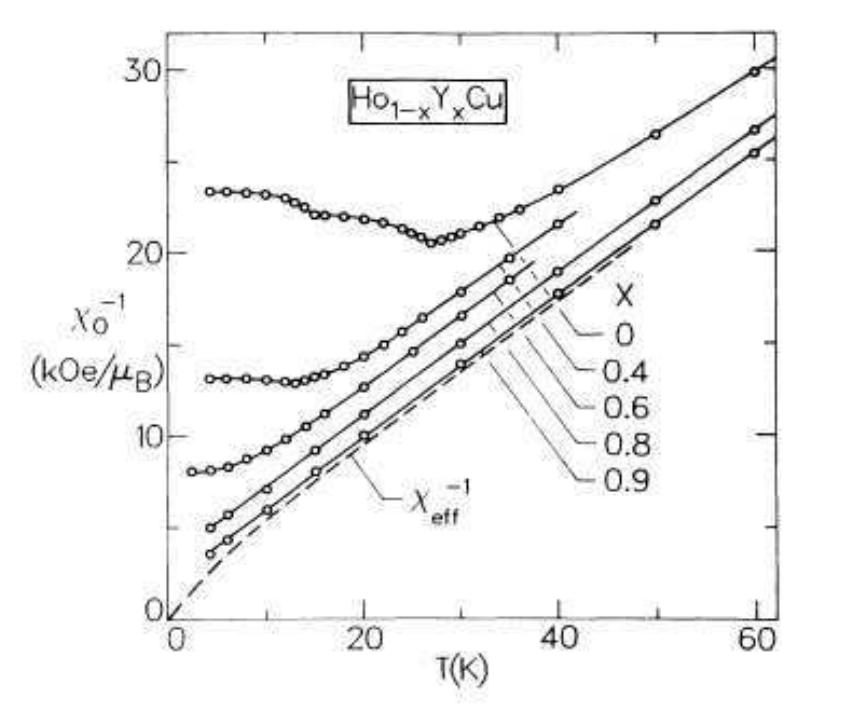
\includegraphics[scale=0.4]{../Fig/SusceptibiliteMagnetique.png}
\end{center}

\tiret{Théorie du champ cristallin}

Dans un modèle plus réaliste, appelé modèle du \og champ cristallin \fg , on ajoute un terme  $A \mu_z^2$ (où $A$ est une constante caractéristique du cristal  qui peut être positive ou négative) dans l'énergie d'un ion de moment magnétique $\Vec{\mu}$ qui devient donc égale à  $A \mu_z^2 -\mu_z B$.

\question Calculer la nouvelle fonction de partition d'un seul ion $z_{CC}(T)$.

\question Calculer le moment magnétique moyen selon $(Oz)$, $M_z$, en fonction de $A, B, k_B T, N$ et $\mu$.

On travaille désormais dans la limite des champs faibles, avec $A>0$.

\question Développer $M_z$ au premier ordre en $\beta \mu B$. En déduire la susceptibilité magnétique
$\chi_M$ du cristal en champ faible. On l'exprimera en fonction de $T, k_B, N, \mu$ et $\exp(\frac{3 \theta_M}{T})$ où $\theta_M=\frac{A \mu^2}{3 k_B}$.

\question Comparer $\chi_M(A >0)$ à $\chi_M(A=0)$ et interpréter.

\question 
\`A partir de l'expression de $\chi_M^{-1}$, montrer que pour $T \gg \theta_M$, $\chi_M^{-1}=\frac{T+\theta_M }{\alpha}$ et expliciter la constante $\alpha$.

\question Les mesures expérimentales de la figure sont-elles compatibles avec le résultat précédent ? Comment pourrait-on en déduire la valeur de $A$ ?

%En déduire des ordres de grandeur de $\theta_M$ et $A$ pour le composé de fraction $x=0.4$.
